%%%%%%%%%%%%%%%%%%%%%%%%%%%%%%%%%%%%%%%%%%%%%%%%%%%%%%%%%%%%%%%%%%%%%%%%%%%%%%%%%%
%%																				%%
%% File name: 		appendicies.tex												%%
%% Project name:	Hochleistungsantenne										%%
%% Type of work:	T3X00 project work											%%
%% Author:			Sarah Brückner, Maximilian Stiefel, Hannes Bohnengel		%%
%% Date:			02nd June 2016												%%
%% University:		DHBW Ravensburg Campus Friedrichshafen						%%
%% Comments:		Created in gedit with tab width = 4							%%
%%																				%%
%%%%%%%%%%%%%%%%%%%%%%%%%%%%%%%%%%%%%%%%%%%%%%%%%%%%%%%%%%%%%%%%%%%%%%%%%%%%%%%%%%

\appendix

\chapter{Batch-Skript: \myemph{rigctld.bat}}
\label{chap:rigctldbat}

\begin{center}
	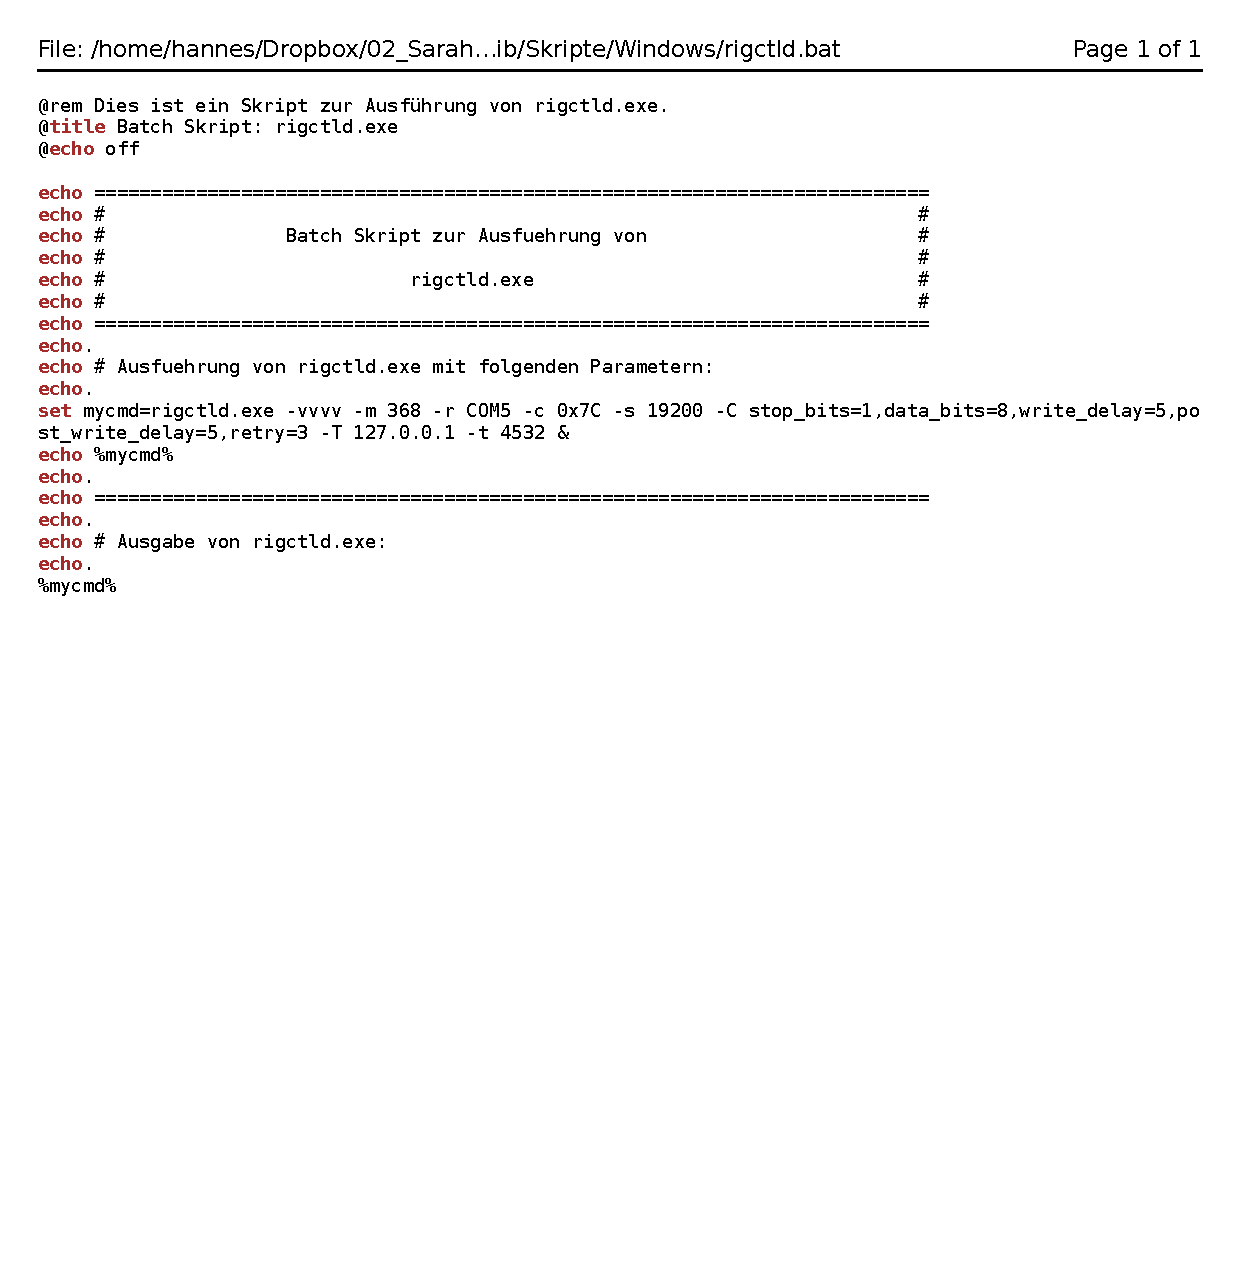
\includegraphics[width=1\textwidth]{./appendicies/rigctld}
\end{center}

\begin{center}
	\Large{\textbf{--- !!! ---}\\AKTUALISIEREN\\\textbf{--- !!! ---}}
\end{center}

%---------------------------------------------------------------------------------

\chapter{Batch-Skript: \myemph{rigctl.bat}}
\label{chap:rigctlbat}

\begin{center}
	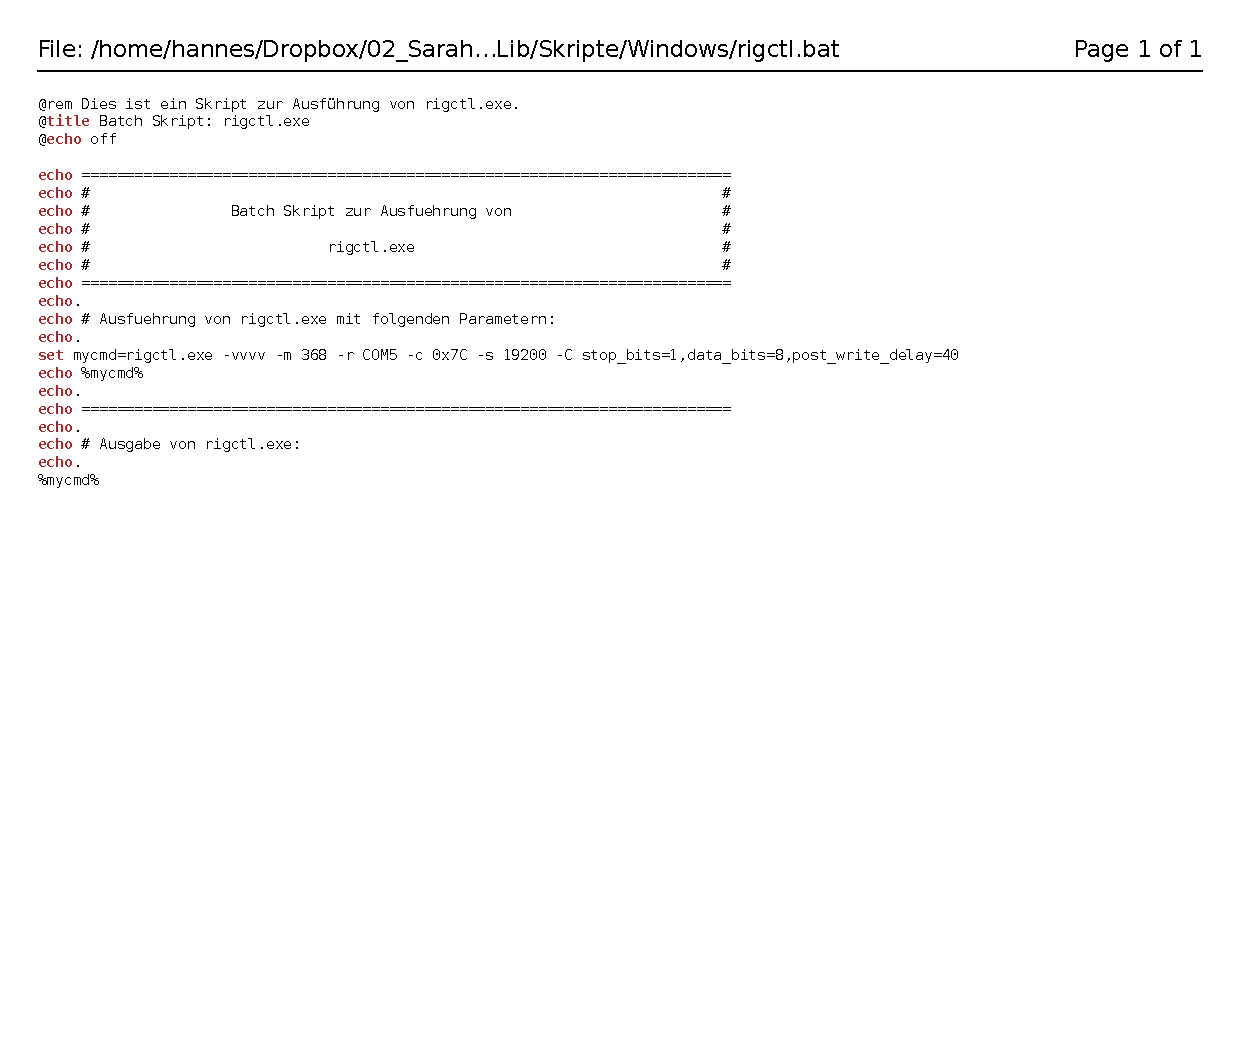
\includegraphics[width=1\textwidth]{./appendicies/rigctl}
\end{center}

\begin{center}
	\Large{\textbf{--- !!! ---}\\AKTUALISIEREN\\\textbf{--- !!! ---}}
\end{center}

%---------------------------------------------------------------------------------

\chapter{Batch-Skript: \myemph{rotctld.bat}}
\label{chap:rotctldbat}

\begin{center}
	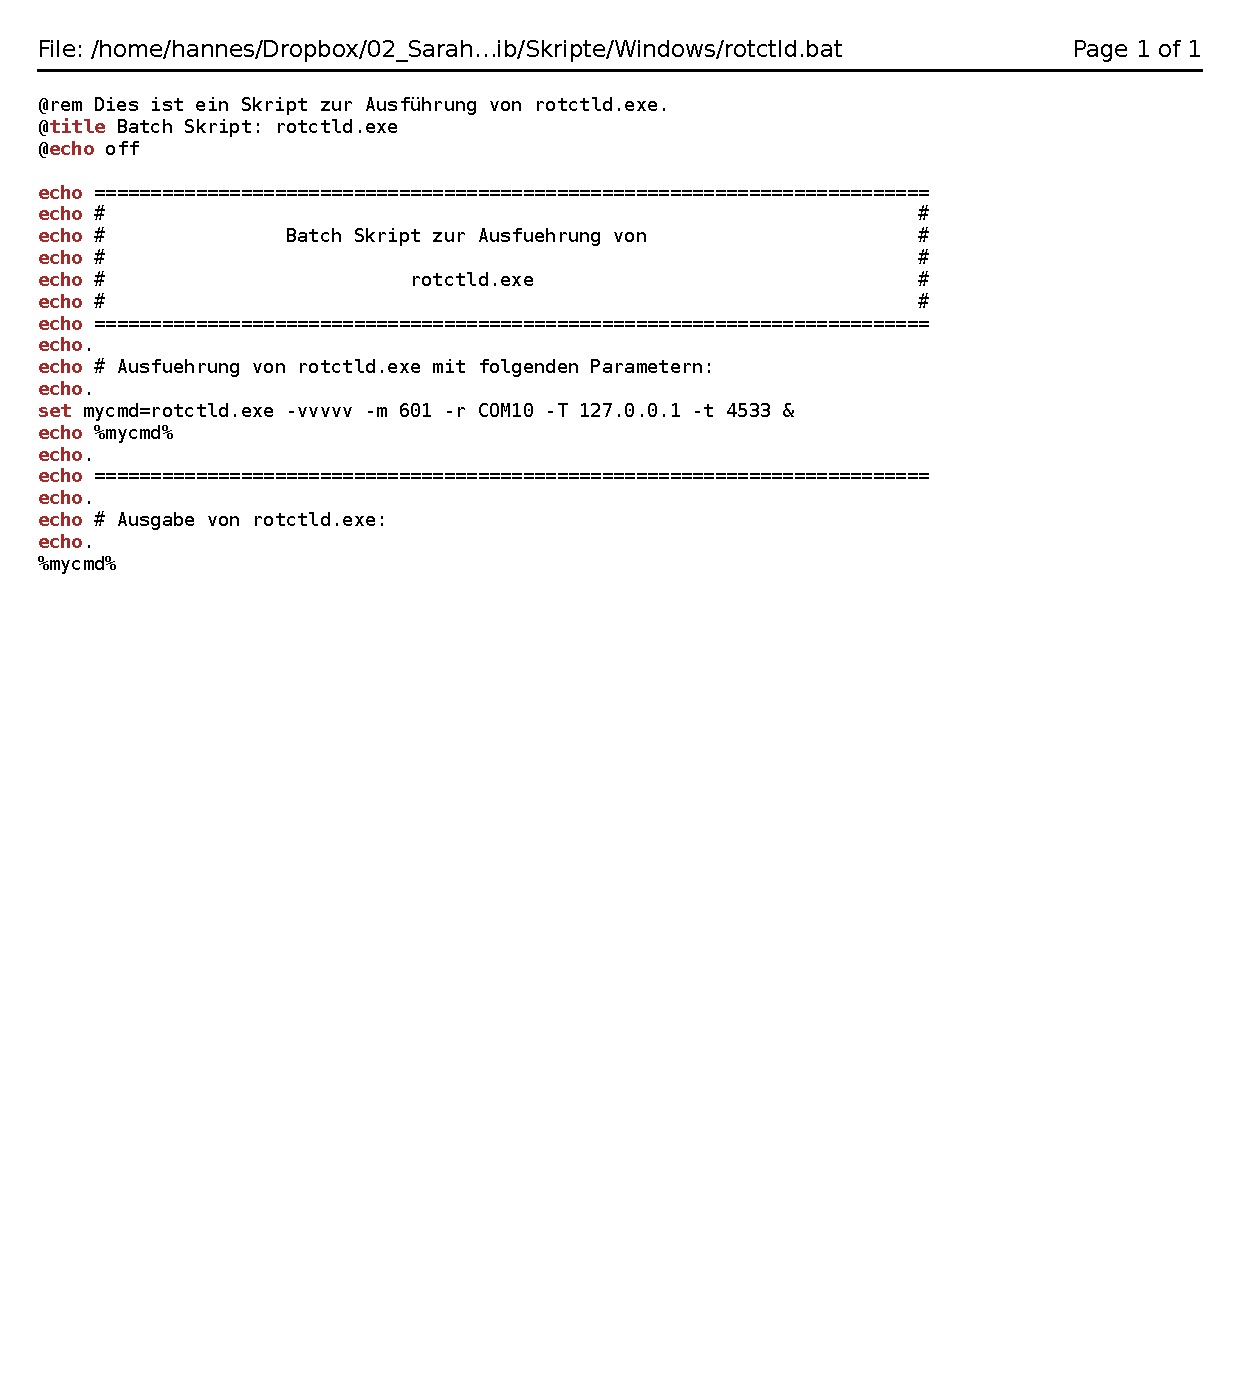
\includegraphics[width=1\textwidth]{./appendicies/rotctld}
\end{center}

\begin{center}
	\Large{\textbf{--- !!! ---}\\AKTUALISIEREN\\\textbf{--- !!! ---}}
\end{center}

%---------------------------------------------------------------------------------

\chapter{Batch-Skript: \myemph{rotctl.bat}}
\label{chap:rotctlbat}

\begin{center}
	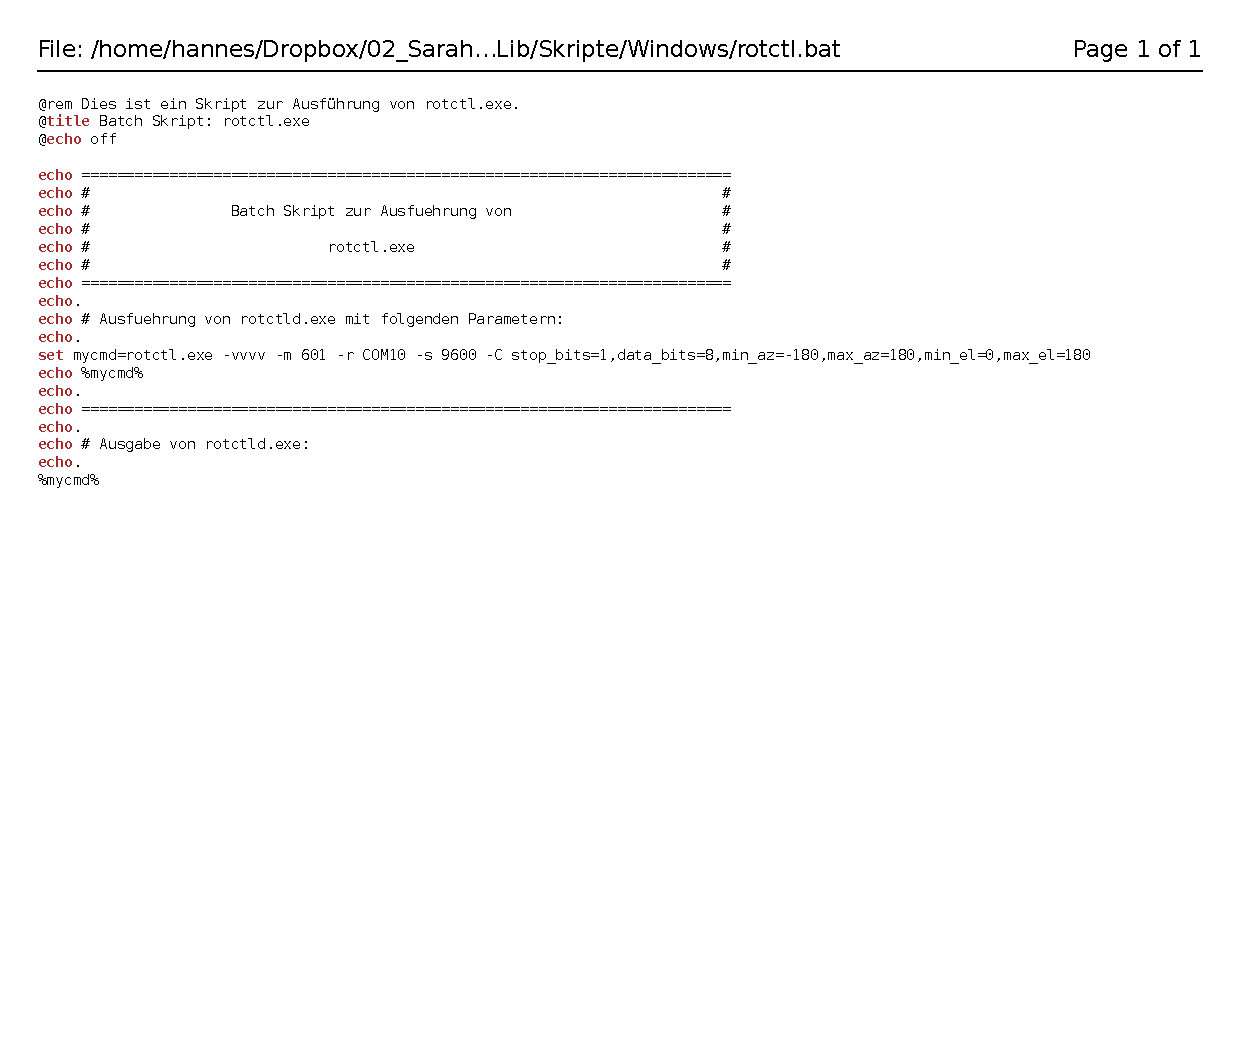
\includegraphics[width=1\textwidth]{./appendicies/rotctl}
\end{center}

\begin{center}
	\Large{\textbf{--- !!! ---}\\AKTUALISIEREN\\\textbf{--- !!! ---}}
\end{center}

%---------------------------------------------------------------------------------

\chapter{Batch-Skript: \myemph{rigctld-dummy.bat}}
\label{chap:rigctlddummybat}

\begin{center}
	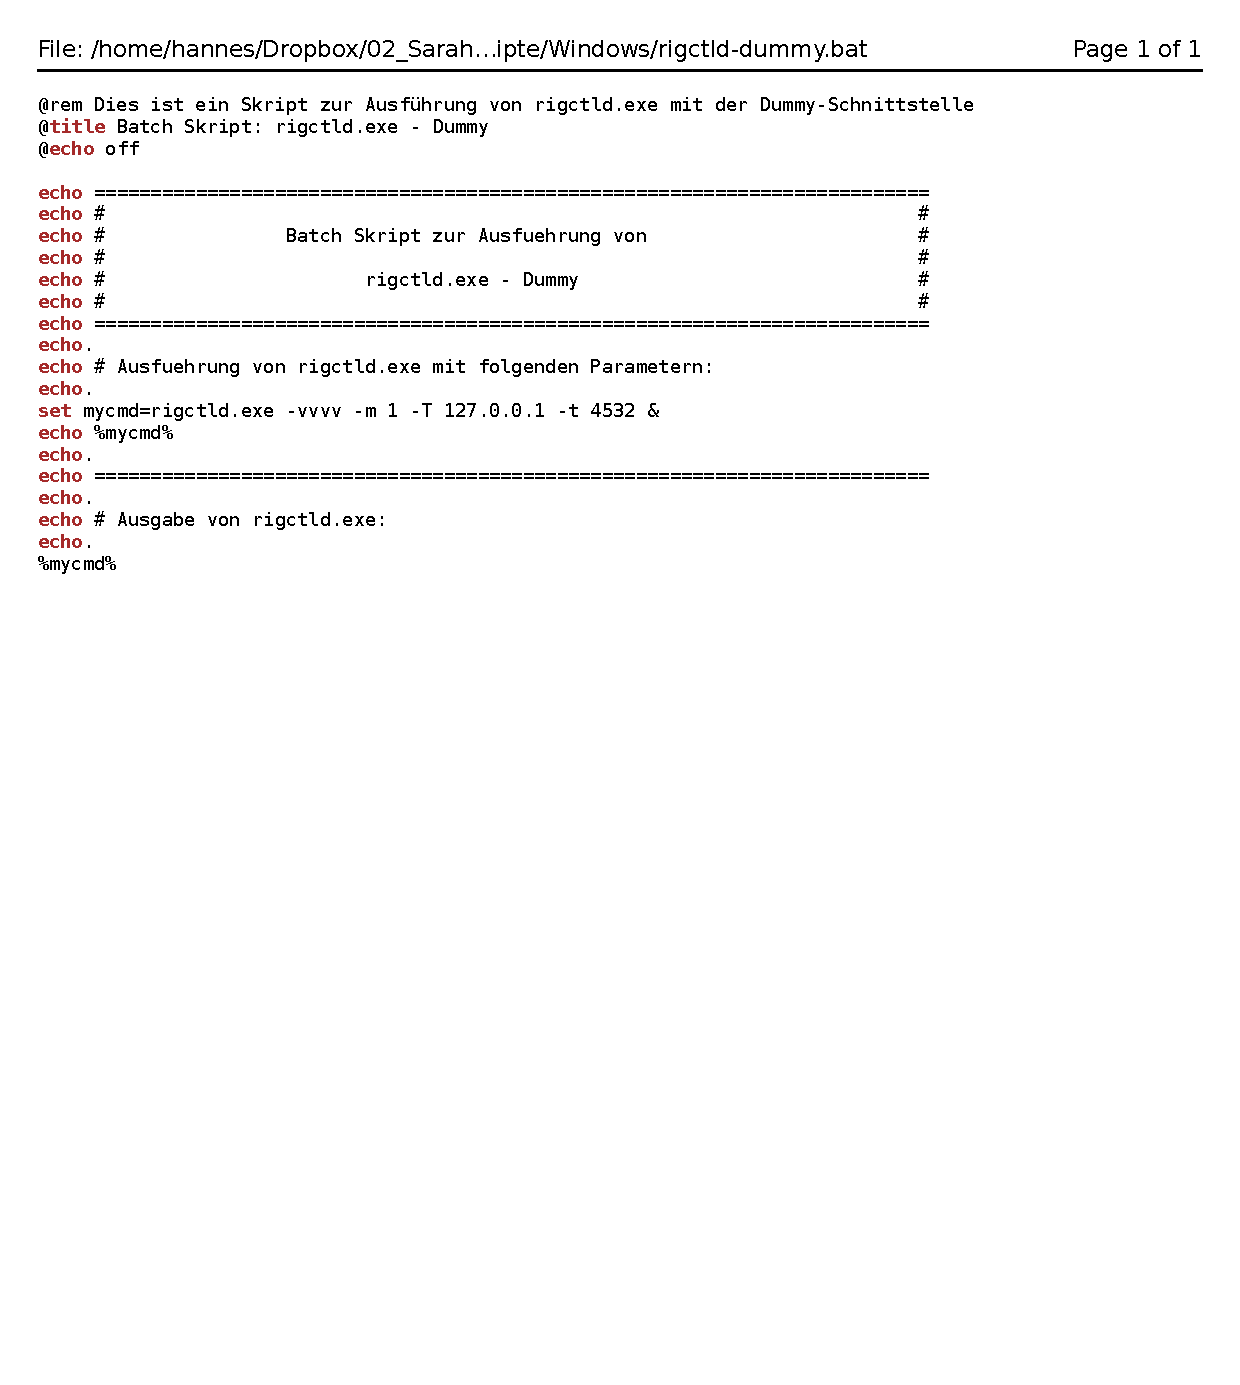
\includegraphics[width=1\textwidth]{./appendicies/rigctld-dummy}
\end{center}

\begin{center}
	\Large{\textbf{--- !!! ---}\\AKTUALISIEREN\\\textbf{--- !!! ---}}
\end{center}

%---------------------------------------------------------------------------------

\chapter{Batch-Skript: \myemph{rotctld-dummy.bat}}
\label{chap:rotctlddummybat}

\begin{center}
	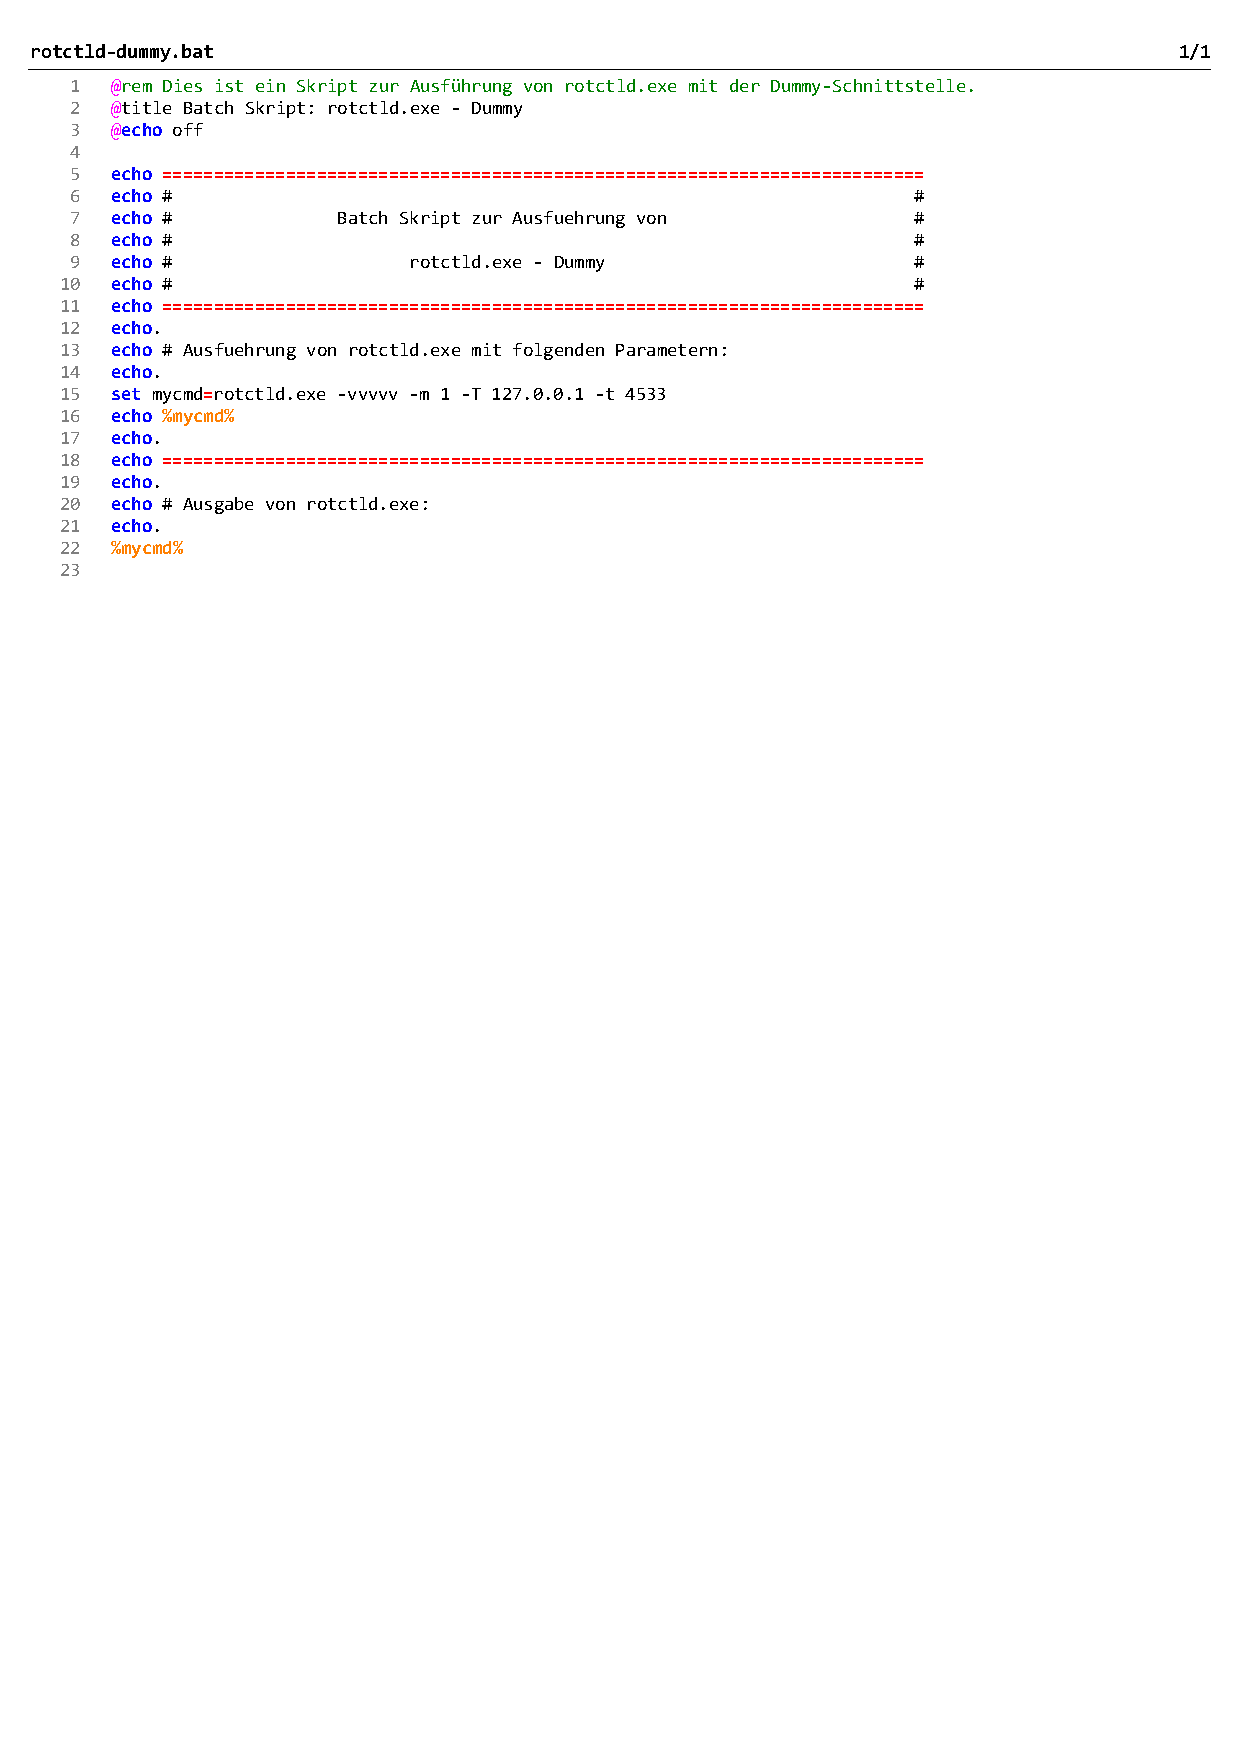
\includegraphics[width=1\textwidth]{./appendicies/rotctld-dummy}
\end{center}

\begin{center}
	\Large{\textbf{--- !!! ---}\\AKTUALISIEREN\\\textbf{--- !!! ---}}
\end{center}

%---------------------------------------------------------------------------------
